\chapter{Searching For Natural SUSY With B-tag Templates.}
\label{chap:templatemethod}


Within this chapter a complimentary technique is discussed as a means to predict the distribution of three and four reconstructed b-quark jets in an event. The recent discovery of the Higgs boson has made third-generation ``Natural \ac{SUSY}'' models attractive, given that light top and bottom squarks are a candidate to stabilise divergent loop corrections to the Higgs boson mass.

Using the $\alphat$ search as a base, a simple template fit is employed to estimate the \ac{SM} background in higher b-tag multiplicities (3-4) from a fit conducted in a low number of reconstructed b-jets (0-2) control region. As a proof-of-concept, the procedure is applied to the SM enriched \mupjets control sample of the \alphat all-hadronic search detailed in Chapter \ref{chap:SUSYsearches}, in both data and simulation. To highlight the relative insensitivity of the choice of b-tagging algorithm working point in the effectiveness of the procedure, results are presented using the \ac{CSV} tagger (introduced in Section (\ref{subsec:cmsobjects-btagging})) for the ``Loose'', ``Medium'' and ``Tight'' working points.

\section{Concept}
\label{sec:templateconcept}

The dominant \ac{SM} backgrounds of most \ac{SUSY} searches are typically \ttbar + jets, W + jets, \zinv + jets or other rare processes with neutrinos in the final state. These processes are characterised by typically having zero or two underlying b-quarks per event. Conversely a third generation squark production signal, such at the \texttt{T1tttt} and \texttt{T1bbbb} models described in the previous chapter, will typically have four underlying b-quarks in its final state.  As \ac{SM} processes with similar topologies are rare, an excess of \nbreco = 3, $\geq$ 4 events would be indicative of a potential natural \ac{SUSY} signature. Therefore the compatibility of the \nbreco distribution in data can be tested via the parameterisation of the \ac{SM} backgrounds in terms of these two most common underlying b-quark topologies. 

 \begin{table}[h!]
\begin{center}
\footnotesize
\begin{tabular*}{0.65\textwidth}{@{\extracolsep{\fill}}cl}
\hline
Typical underlying b-quark content & Process \\
\hline\hline
 = 0 & $W \rightarrow l\nu$  + jets \\
   & \zinv  + jets  \\
   & $Z/\gamma^{*} \rightarrow \mu\mu$ + jets \\
 \\
 = 1 & $t$ + jets  \\
 \\
= 2 & \ttbar + jets
\end{tabular*}
\end{center}
\caption[Typical underlying b-quark content of different \ac{SM} processes which are common to many \ac{SUSY} searches.]{Typical underlying b-quark content of different \ac{SM} processes which are common to many \ac{SUSY} searches.}
\end{table}

Thus two templates are defined, Z0 and Z2 (single top processes are a negligible background, $\sim 1\%$ within the \alphat search, and are combined together with \ttbar) which represent processes which have an underlying b-quark content of zero or two respectively. 

Both these templates are generated through the application of the relevant event selection, and can then be taken from the underlying $n_{b}^{reco}$ distribution directly from simulation. However as discussed within Section (\ref{subsec:backgroundestimation}), there are large uncertainties for high $n_{b}^{reco}$ multiplicities due to limited MC statistics. This is particularly prominent for the Z0 templates, where events with a large number of reconstructed b-tags jets are driven primarily by the mis-tagging of light-quarks. Within both the medium and tight working point of the \ac{CSV} tagger, the expected mis-tagging rate is only around 1 and 0.1\% respectively, leading to large uncertainties in the template shape in this region. Therefore to improve the statistical precision of the predictions within the signal region, the formula method introduced in Section (\ref{subsec:formulamethod}) is used. 

The generation of the template shapes, are dependant upon the jet-flavour content and b-tagging rate within the phase space of interest, with the tagging probabilities of a jet being a function of the jet \pt, the pseudo-rapidity $\rvert\eta\lvert$, and jet-flavour. This can be observed in Figure \ref{fig:templatetaggingefficiencies}, where the b-tagging / c-quark mis-tagging / light mis-tagging efficiency for the three working points of the \ac{CSV} tagger are shown as a function of jet \pt. 

\begin{figure}[ht]
\centering
\begin{minipage}[b]{0.48 \linewidth}
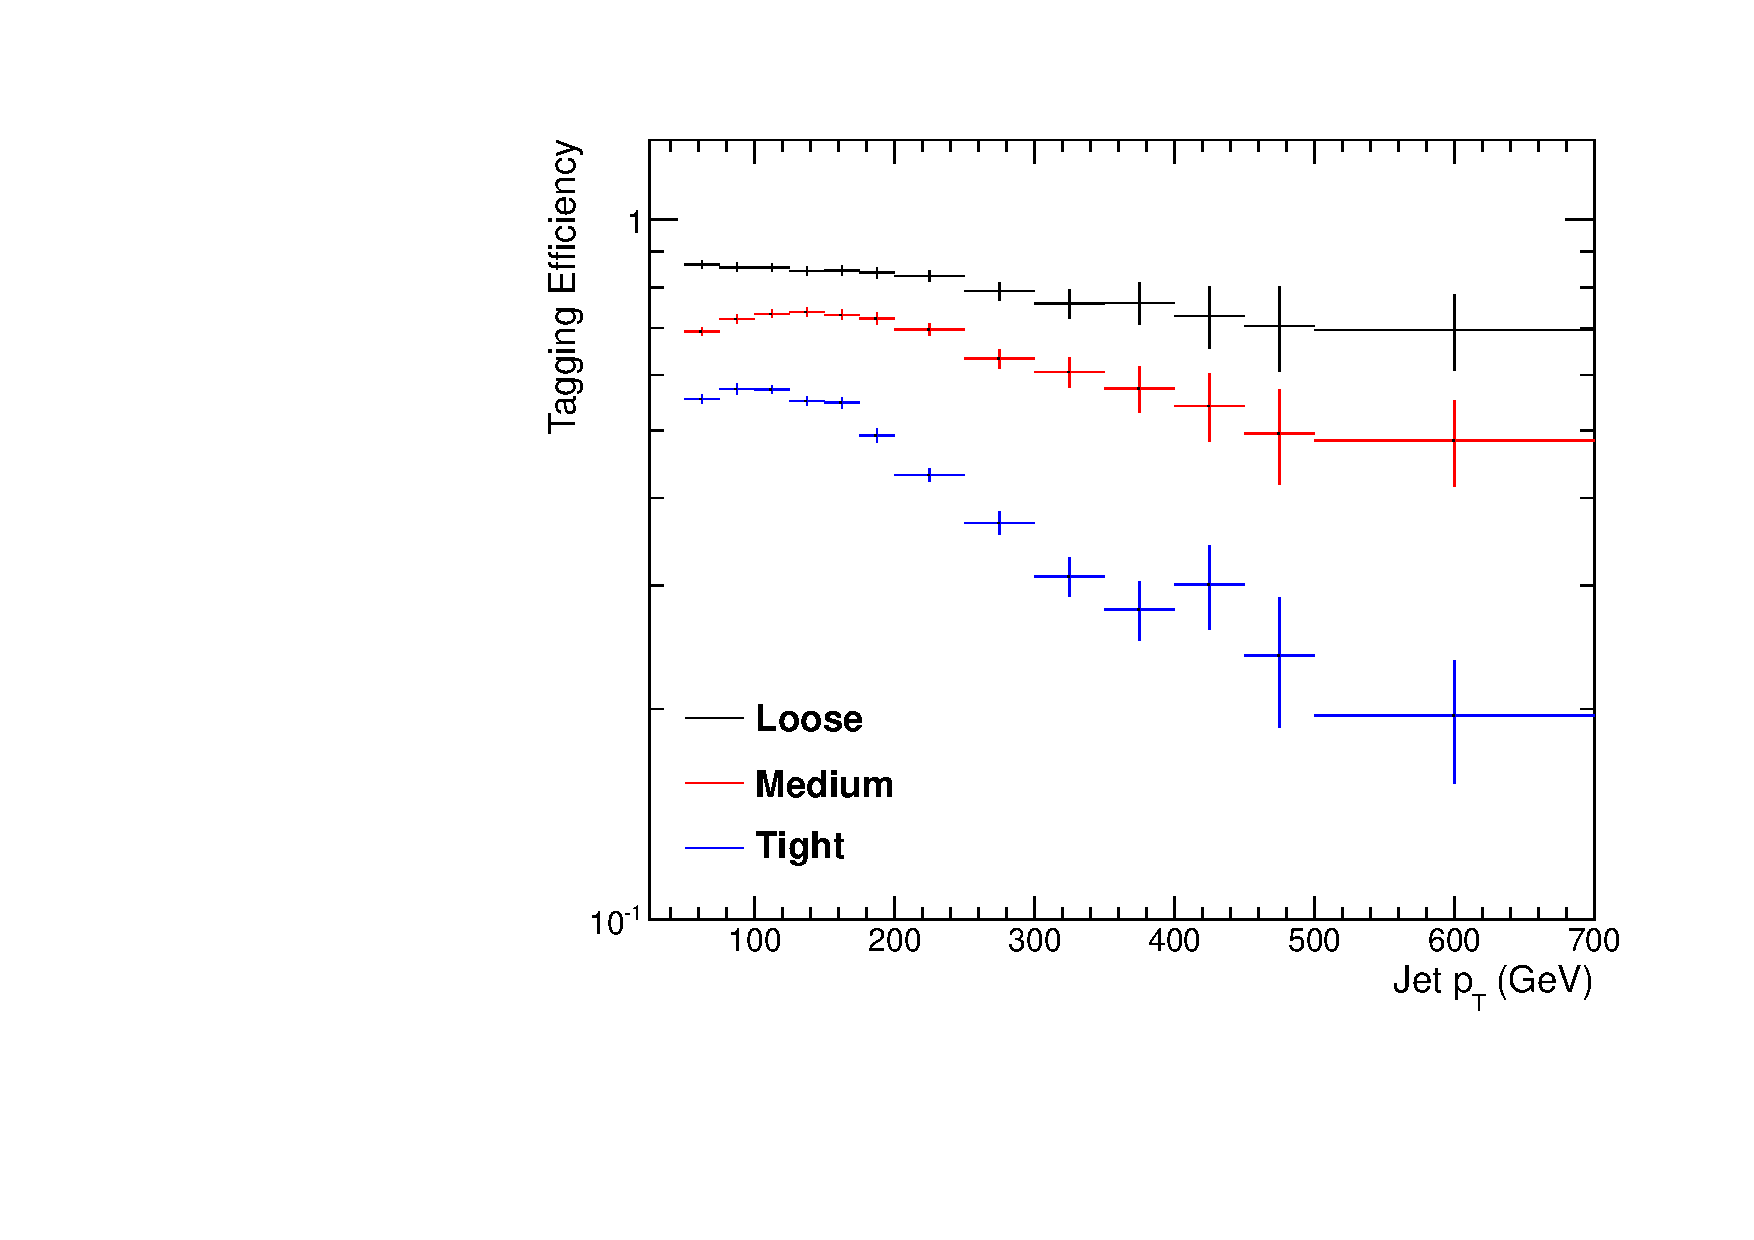
\includegraphics[width = 1.0\linewidth]{plots/bjet_PtDistribution_Htbin_Template_375.pdf}
\centering (a)  b-jets
\end{minipage}
\quad
\begin{minipage}[b]{0.48\linewidth}
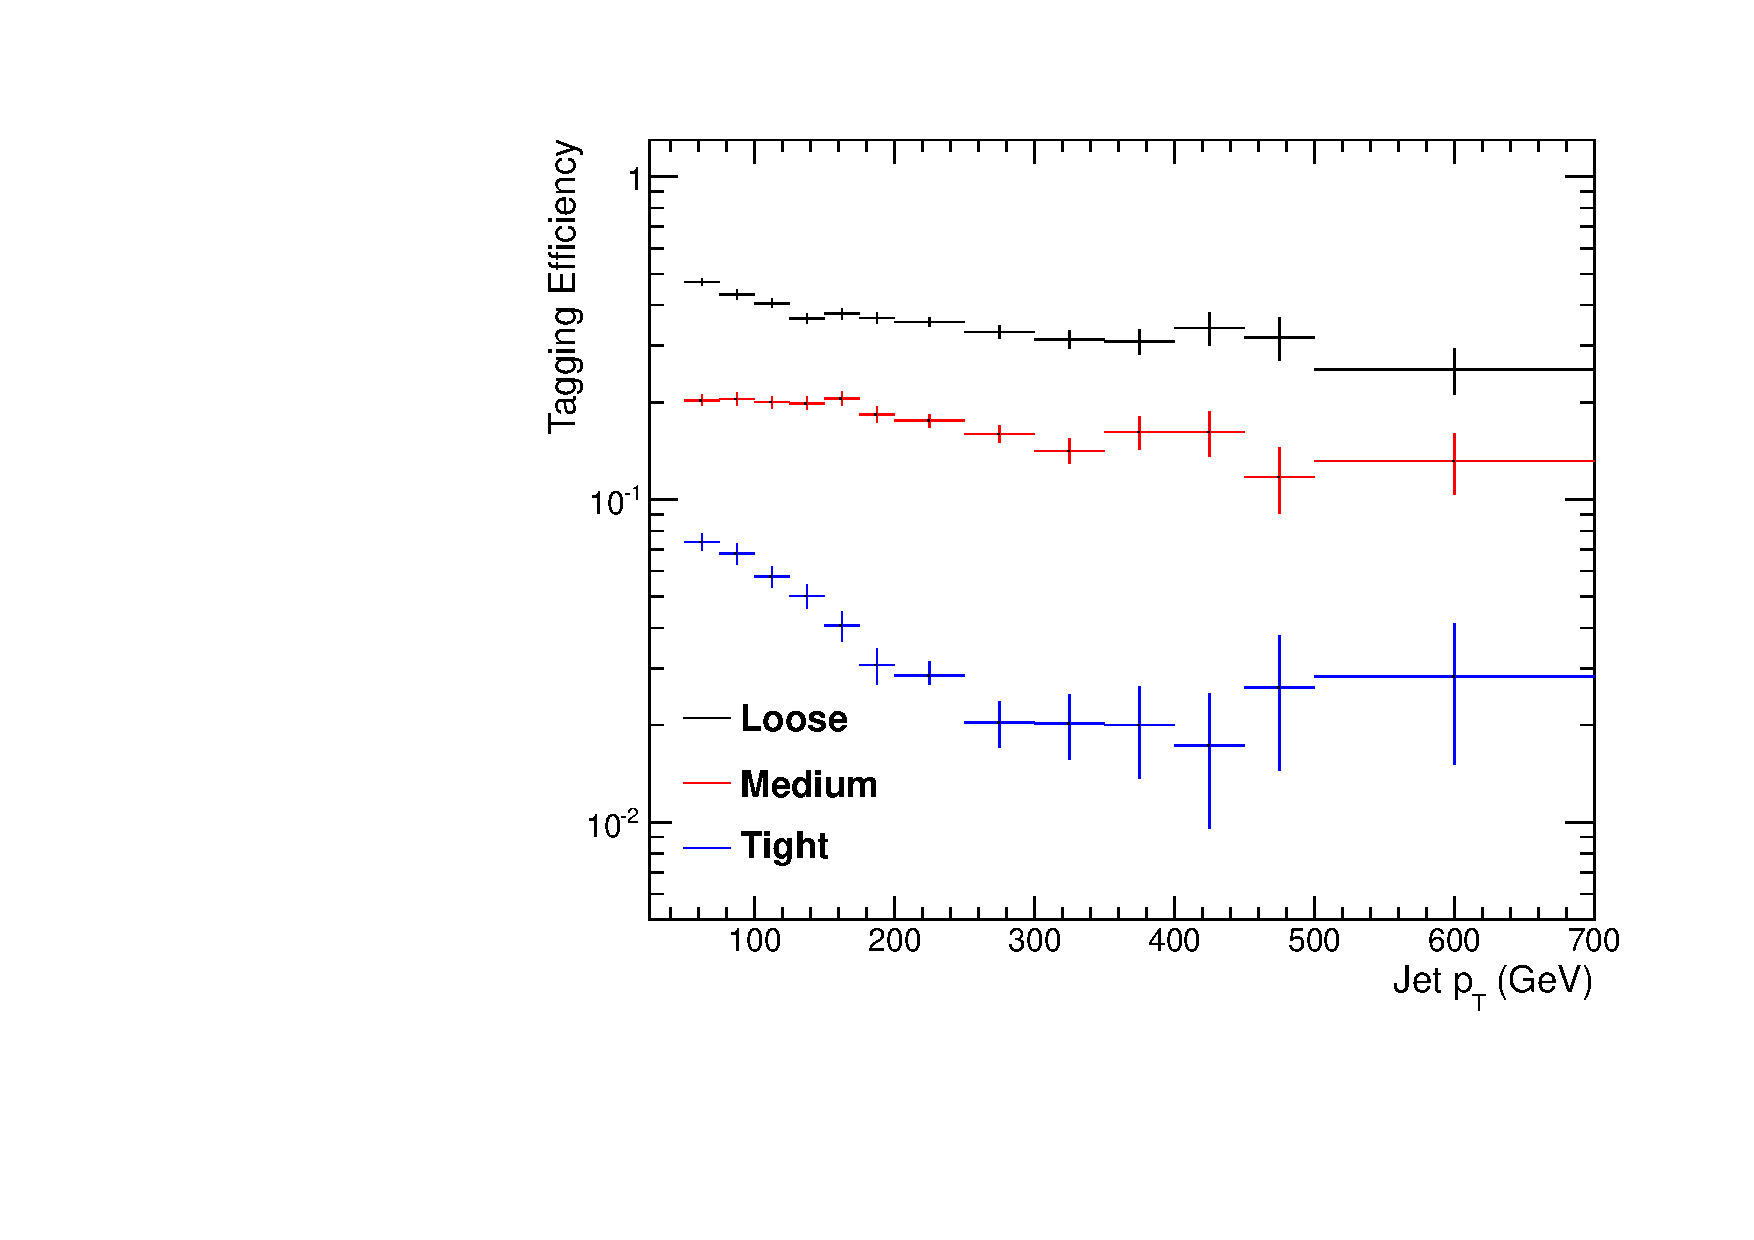
\includegraphics[width = 1.0\linewidth]{plots/cjet_PtDistribution_Htbin_Template_375.pdf}
\centering (b) c-jets
\end{minipage}
\quad
\begin{minipage}[b]{0.48\linewidth}
\centering
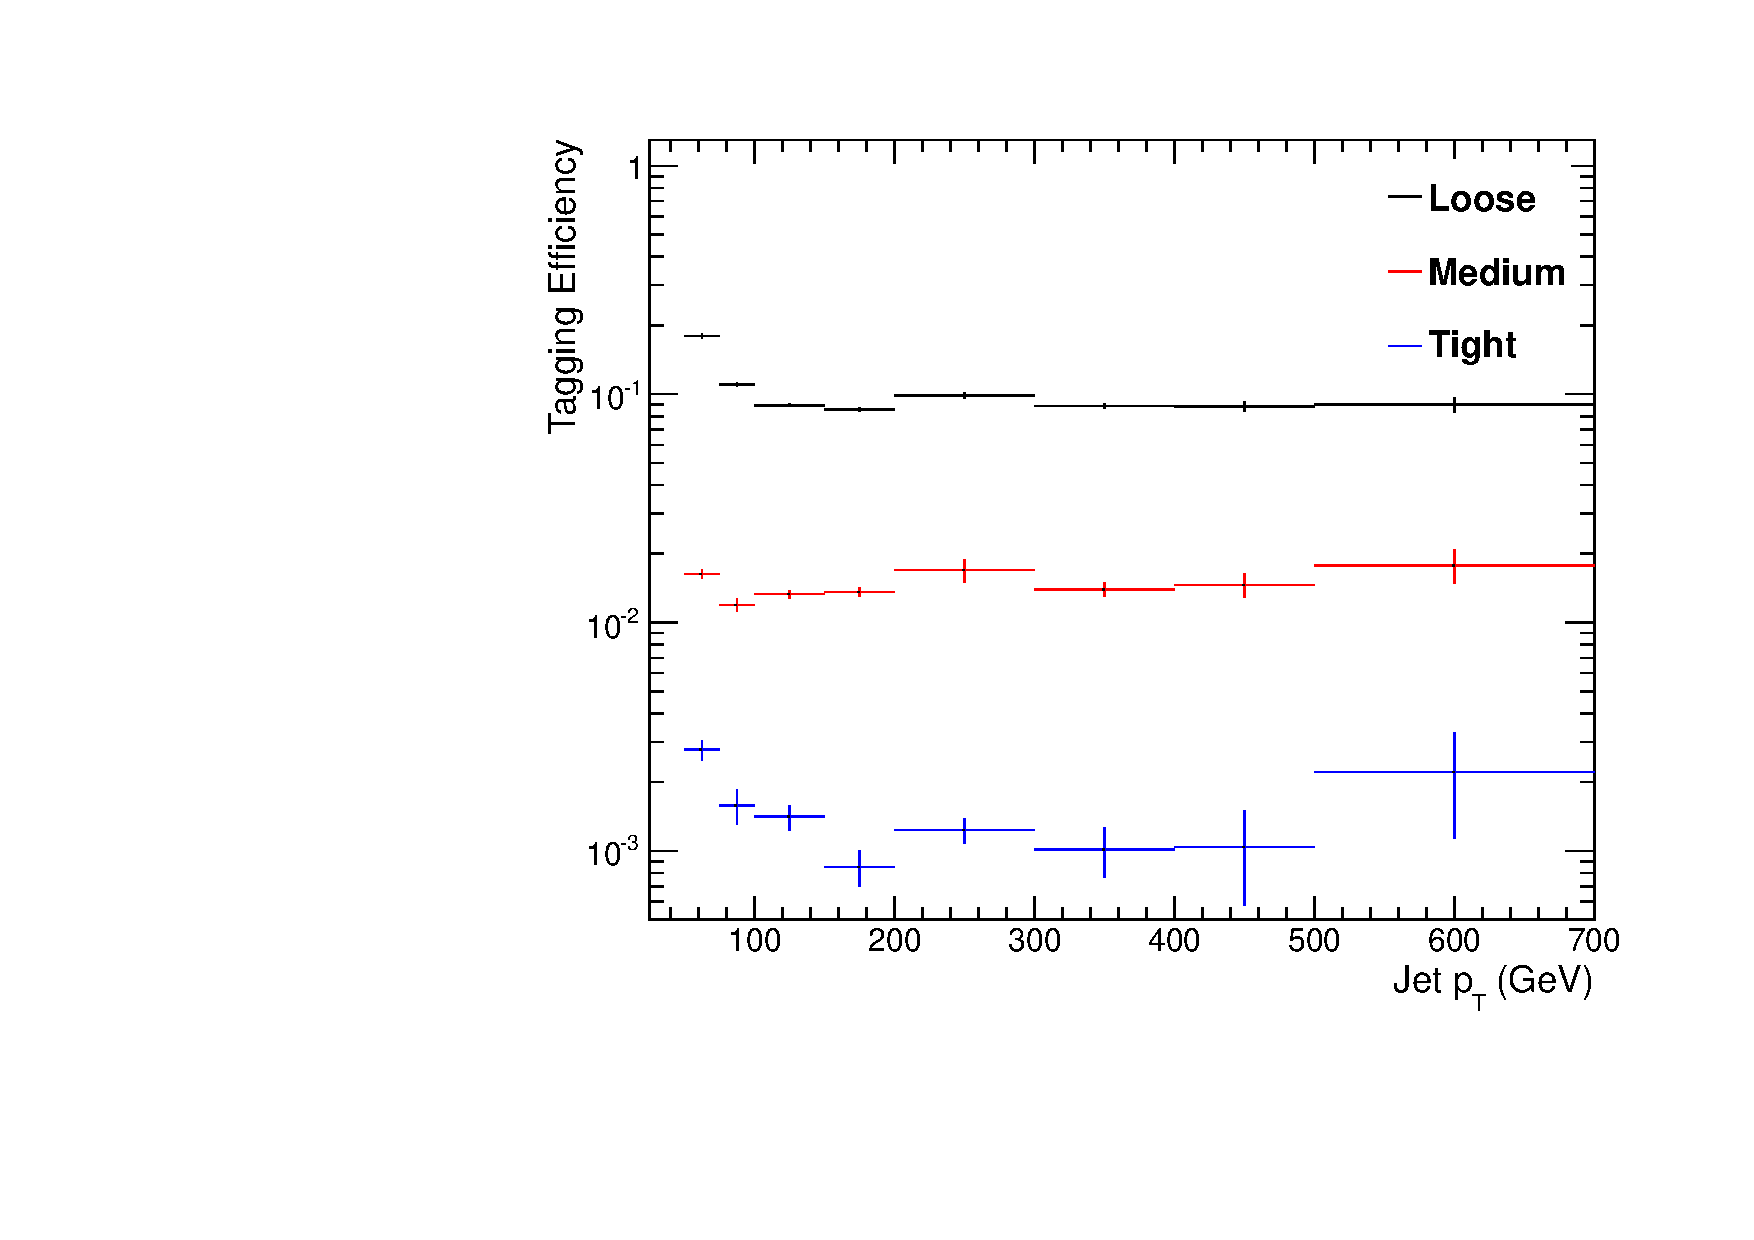
\includegraphics[width = 1.0\linewidth]{plots/lighjet_PtDistribution_Htbin_Template_375.pdf}
\centering (c) light-jets
\end{minipage}
\caption[The b-tagging (a), c-quark mis-tagging (b), and light-quark mis-tagging rate (c$)$ as measured in simulation after the \alphat analysis, \mupjets control sample selection in the region \theht $>$ 375.]{The b-tagging (a), c-quark mis-tagging (b), and light-quark mis-tagging rate (c$)$ as measured in simulation after the \alphat analysis, \mupjets control sample selection in the region \theht $>$ 375.}
\label{fig:templatetaggingefficiencies}
\end{figure}

Before the template shapes are determined and applied to data, the relevant jet \pt and \eta corrections are applied to correct the measured b-tagging rate in simulation to that of data, as specified in Section (\ref{subsec:formulamethodsf}), which propagate through to the average determined b-tagging rates per analysis \theht bin, as in the \alphat analysis.  

These two template shapes once generated from simulation, can then be fitted to data in a low $n_{b}^{reco}$ control region (0-2), by allowing the normalisation constants $\theta_{Z0}$ and $\theta_{Z2}$ of the two templates to float. The best fit values of $\theta_{Z0}$ and $\theta_{Z2}$ are used, along with the knowledge of the template shapes, to extrapolate an estimate in the high $n_{b}^{reco}$ signal region (3,4), which is then compared to what is observed in data. Any large excess in data compared to the template prediction would indicate that the \nbreco distribution is not adequately described by the \ac{SM} backgrounds which compose the templates. This method can, in principle, be applied to any analysis where the signal hypothesis has a larger underlying b-quark spectra than the \ac{SM} backgrounds, as it solely relies on fitting to the shape of the $n_{b}^{reco}$ distribution. 

However in the scenario where a \ac{SUSY} signal sits at a low number of underlying b-quarks, the template would be unable to discriminate between this signal and background and would be accommodated within the fit in the control region. This will be the case unless the jet \pt distribution of the signal and background were drastically different, in which case there would, anyway be many more sensitive ways to establish the presence of a signal in the data than this method. Indeed the template method is only really applicable to the hypothesis that any signal resides at high \nbreco and that the control region 0 $\geq \nbreco \leq 2$ is indeed signal free.  



\section{ Application to the \alphat Search}
\label{sec:templateapplication}

As detailed in the previous chapter, the \alphat analysis is a search for \ac{SUSY} particles in all-hadronic final states, utilising the kinematic variable \alphat to suppress QCD to a negligible level. \ac{SM} enriched control samples are used to estimate the background within an all-hadronic signal region. 

The selection for the \mupjets control samples defined in Section (\ref{subsec:controlsampledefinition}) is used to demonstrate the template fitting procedure both conceptually in simulation, and also when applied in data. This is chosen, as such a selection is dominated by events stemming from the \ac{SM} processes with little or no signal contamination from potential new physics. Neither are contributions from rare \ac{SM} processes with a higher underlying b-quark content (e.g. $t\bar{t}b\bar{b}$) expected. For these reasons, there is a degree of confidence that the procedure should adequately describe the observations in data when extrapolated to the signal region.

The analysis presented here is binning in source jet multiplicity bins, of 3, 4 and $\geq$ 5 reconstructed jets per event (di-jet events are not included as there is no contribution to the high $n_{b}^{reco}$ region (3,4)) , in order to reduce the kinematic jet \pt dependence. Furthermore the analysis is split into three \theht regions, 

\begin{itemize}
\item 275-325 \GeV
\item 325-375 \GeV
\item $>$ 375 \GeV
\end{itemize}

contrary to the eight used within the \alphat analysis. Templates for both underlying b-quark content hypotheses are then generated for the nine defined analysis bins.

\subsection{Proof of principle in simulation}
\label{subsec:templateclosuretest}

In order to demonstrate that the template procedure produces accurate predictions within simulation, the simulation samples in the analysis are firstly split into two to allow for statistically independent fits to be performed. 

By combining the relevant ingredients necessary to employ the formula method, \nbreco templates for Z = 0 and Z= 2 are generated individually for each \njet and \theht bin using one half of each simulation sample. A fit of these two templates is then performed in the low \nbreco (0-2) region, back to the sum of the other halves of each simulation sample in order to check that the relevant information can be recovered in the \nbreco signal region (3-4).

The fits are performed independently within each of the defined analysis bins to reduce the dependence of the shapes of these distributions on simulation. The half of the simulation sample for which the templates are fitted too, are taken directly from simulation, extending this procedure to also be a validation of the formula method in accurately describing the $n_{b}^{reco}$ distribution within the control region itself. Additionally as this test is performed in simulation, the relevant corrections of the b-tagging rates between data and simulation are \emph{not} applied.  

Within Figure \ref{fig:template_closure_njet5}, the results of this fitting procedure are shown for each \ac{CSV} working point. Results are presented for the $\njet \geq 5$ category, using the \mupjets control sample selection in the inclusive \theht$>$ 375 \GeV analysis bin. The grey bands represent the statistical uncertainty on the template shapes. Additional fits are shown for other \njet categories can be found within Appendix \ref{app:templatemc}. 

Furthermore the extrapolated fit predictions within the high $n_{b}^{reco}$ signal region, are summarised for all \theht bins and working points in Table \ref{tab:template_mctable}. 

\begin{table}[h!]
\begin{center}
\footnotesize
\begin{tabular*}{0.95\textwidth}{@{\extracolsep{\fill}}lccc}
\cline{1-4}
\multicolumn{1}{c}{\theht} & 275-325 & 325-375 & $>$375 \\

\multicolumn{4}{c}{Loose working point} \\
\hline\hline
Simulation $n_{b} = 3$ & $793.0 \pm 14.8$ & $387.9 \pm 10.2$ & $794.1 \pm 14.34$ \\
Template $n_{b} = 3$ & $820.4 \pm 26.7$ & $376.3 \pm 11.9$ & $780.1 \pm 15.1$ \\
Simulation $n_{b} = 4$ & $68.2 \pm 3.9$ & $27.6 \pm 2.7$ & $91.28 \pm 4.9$ \\
Template $n_{b} = 4$ & $72.5 \pm 4.7$ & $28.25 \pm 2.34$ & $84.4 \pm 3.8$ \\
\hline
\multicolumn{4}{c}{Medium working point} \\
\hline\hline
Simulation $n_{b} = 3$ & $133.7 \pm 5.7$ & $74.5 \pm 4.5$ & $164.2 \pm 6.4$ \\
Template $n_{b} = 3$ & $132.8 \pm 4.8$ & $74.5 \pm 3.9$ & $159.9 \pm 5.7$ \\
Simulation $n_{b} = 4$ & $1.6 \pm 0.6$ & $0.6 \pm 0.4$ & $3.4 \pm 0.9$ \\
Template $n_{b} = 4$ & $1.8 \pm 0.2$ & $1.1 \pm 0.2$ & $4.1 \pm 0.4$ \\
\hline
\multicolumn{4}{c}{Tight working point} \\
\hline\hline
Simulation $n_{b} = 3$ & $26.9 \pm 2.6$ & $13.9 \pm 1.9$ & $31.8 \pm 2.9$ \\
Template $n_{b} = 3$ & $24.7 \pm 1.5$ & $13.8 \pm 1.2$ & $28.1 \pm 1.5$ \\
Simulation $n_{b} = 4$ & $0.5 \pm 0.4$ &  -  & - \\
Template $n_{b} = 4$ & $0.1 \pm 0.1$ & $0.1 \pm 0.1$ & $0.2 \pm 0.1$ \\
\end{tabular*}
\end{center}
\caption[Summary of the fit predictions in the $n_{b}^{reco}$ signal region for $n_{jet} = 3, = 4, \geq 5$. The fit region is $n_{b}^{reco}$ = 0, 1, 2 and simulation yields are normalised to an integrated luminosity of 10 fb$^{-1}$. ]{Summary of the fit predictions in the $n_{b}^{reco}$ signal region for $n_{jet} = 3, = 4, \geq 5$. The fit region is $n_{b}^{reco}$ = 0, 1, 2 and simulation yields are normalised to an integrated luminosity of 10 fb$^{-1}$. The uncertainties quoted on the template yields are purely statistical.}\label{tab:template_mctable}
\end{table}

The pull distributions for all the fits performed can be found in Appendix \ref{app:templatepulldistributions}, and are compatible with a mean of zero and standard deviation of one, showing no obvious bias to the fitting procedure. The good overall agreement summarised in the table validates both the formula method used to generate the templates as well as the method of extrapolation to the high \nbreco signal region. The application of this method to the same selection in a data control sample, is now used to demonstrate necessary control over the efficiency and mis-tagging rates when b-tagging scale factors are applied, and to test the assumption of no signal contamination with the \mupjets control sample.

\begin{minipage}{\linewidth}
\footnotesize
\vspace{5mm}
\centering
\begin{minipage}{.51\textwidth}
\centering
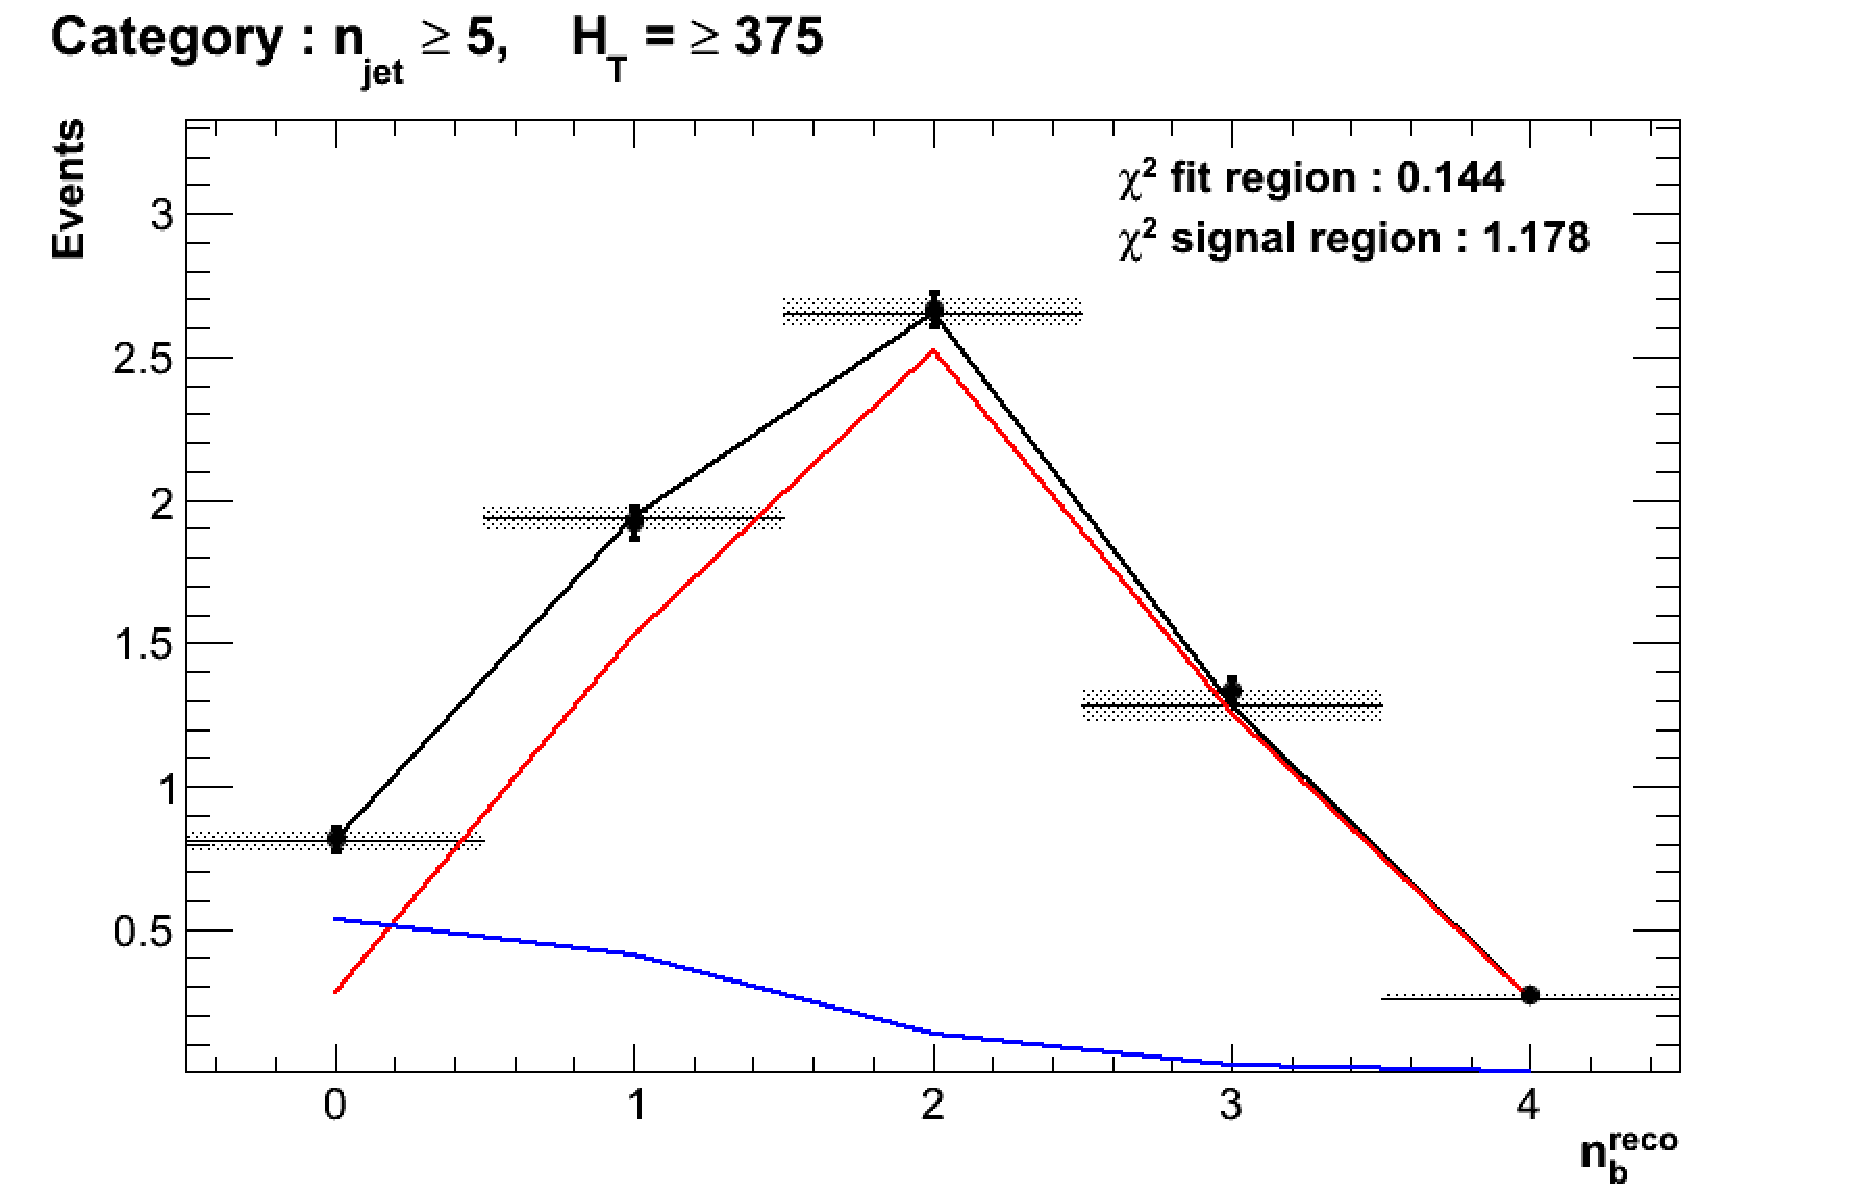
\includegraphics[width = 1.0\linewidth]{plots/ThesisPlots/Final_Fit_To_MC_Normal_Loose_HTBin_OneMuon_Template_375_jet_mult_5.pdf}
\centering (a) Loose working point : $n_{jet} \geq$  5 
\end{minipage}
\end{minipage}

\xspace

\begin{figure}[ht]
\footnotesize
\centering
\begin{minipage}[b]{0.51\linewidth}
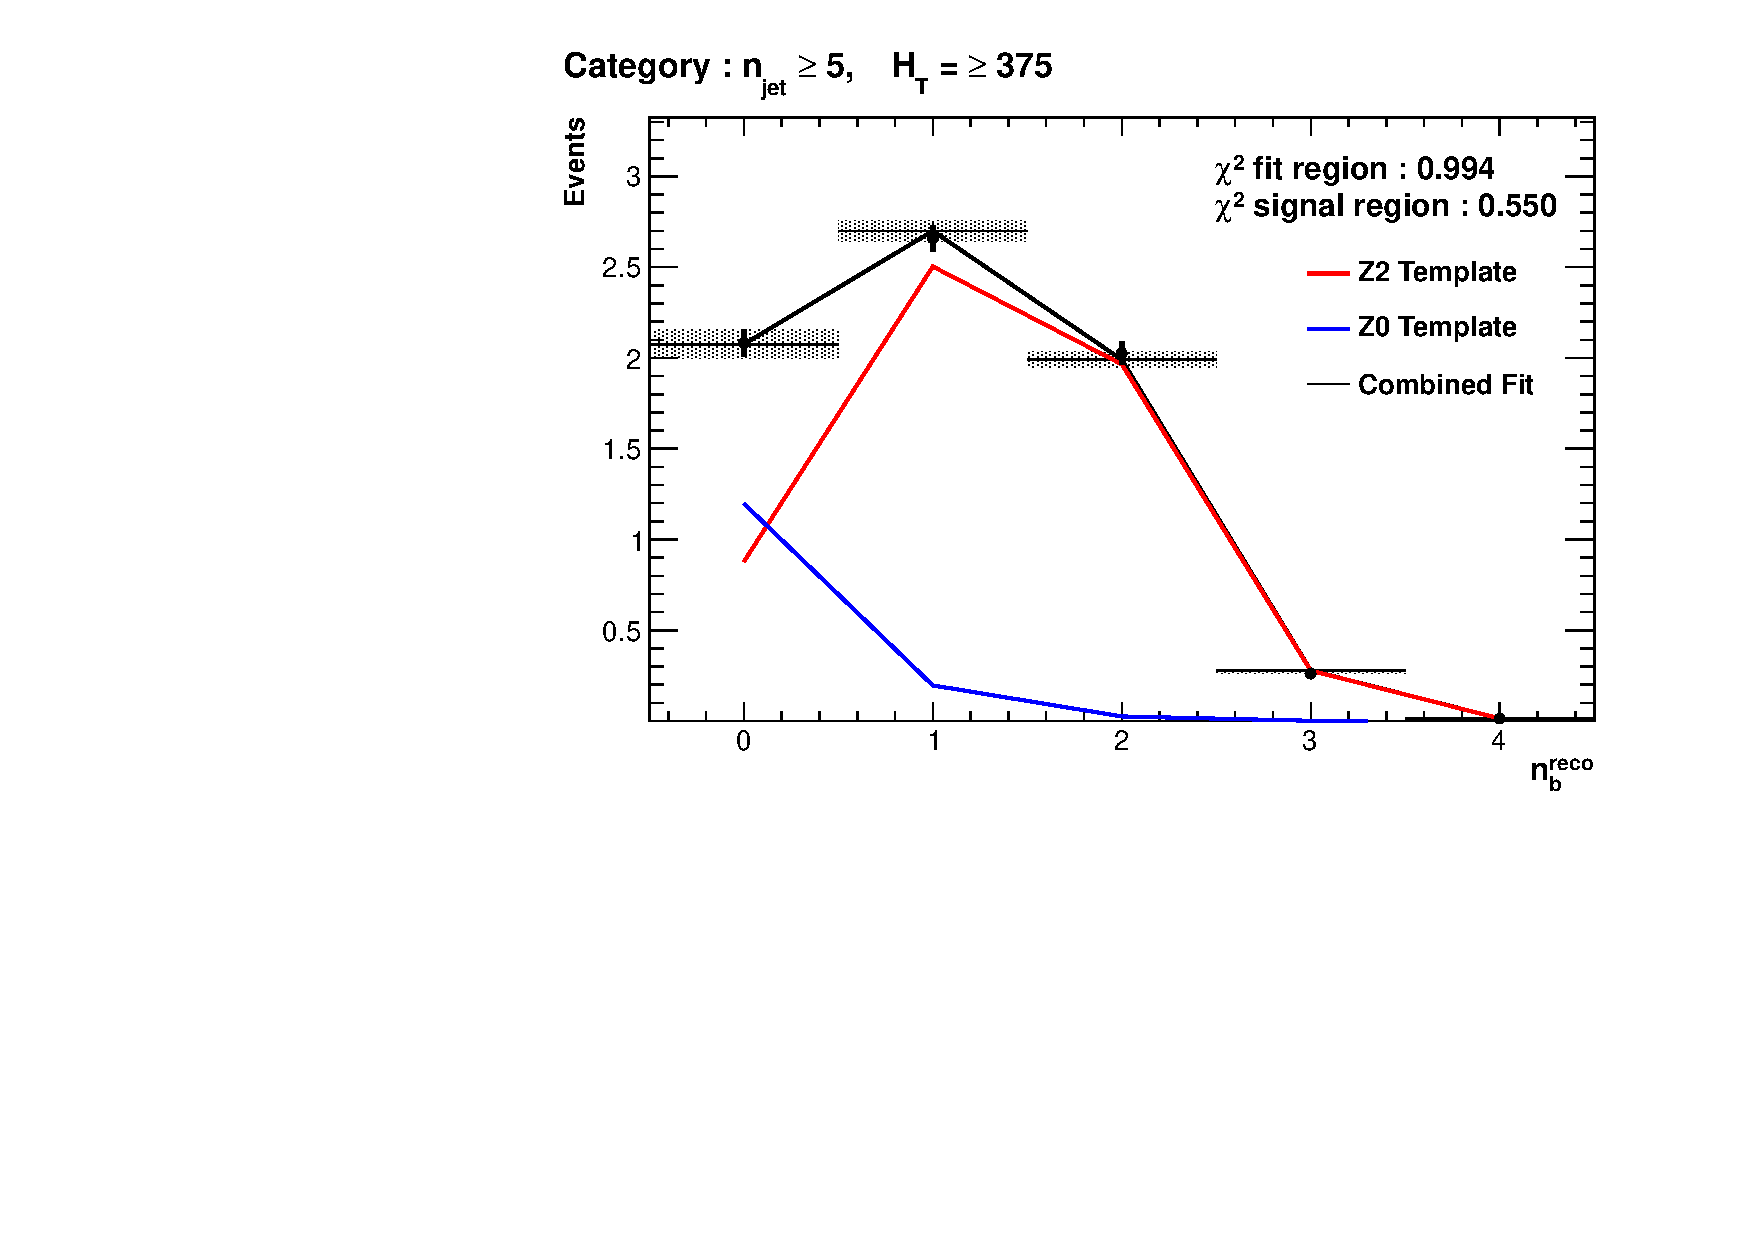
\includegraphics[width = 1.0\linewidth]{plots/ThesisPlots/Final_Fit_To_MC_Normal_Medium_HTBin_OneMuon_Template_375_jet_mult_5.pdf}
\centering (b) Medium working point : $n_{jet} \geq$ = 5 
\end{minipage}
\quad
\begin{minipage}[b]{0.51\linewidth}
\centering
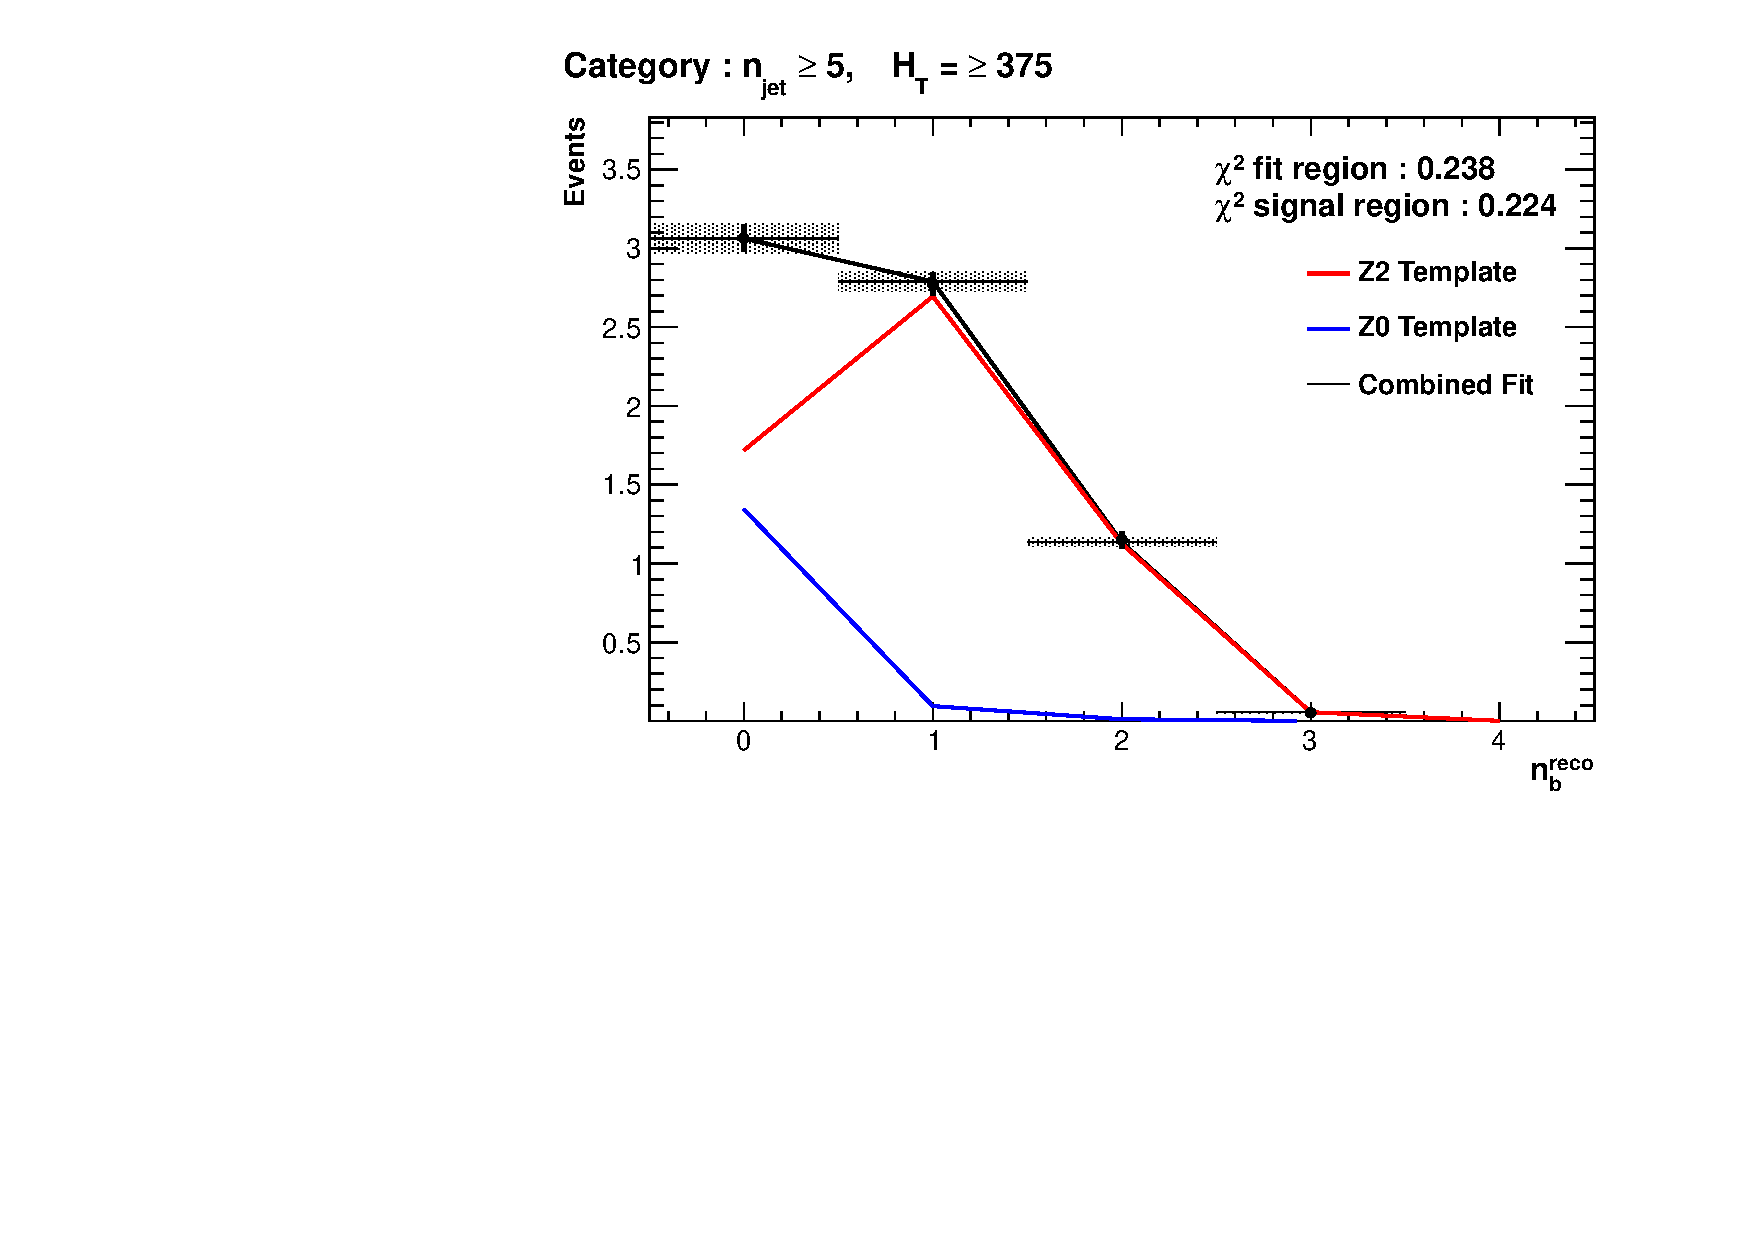
\includegraphics[width = 1.0\linewidth]{plots/ThesisPlots/Final_Fit_To_MC_Normal_Tight_HTBin_OneMuon_Template_375_jet_mult_5.pdf}
\centering (c) Tight working point : $n_{jet} \geq$ 5 
\end{minipage}
\caption[The results of fitting the Z = 0 and Z = 2 templates to the $n_{b}^{reco}$ = 0, 1, 2 bins taken directly from simulation in the region \theht $>$ 375 \GeV, for the $n_{jet} \geq 5$ category.]{The results of fitting the Z = 0 and Z = 2 templates to the $n_{b}^{reco}$ = 0, 1, 2 bins taken directly from simulation in the region \theht $>$ 375 \GeV, for the $n_{jet} \geq 5$ category. The blue template represents Z = 0, while the red template represents Z = 2. Grey bands represent the statistical uncertainty of the fit. The $\chi^{2}$ parameter displayed represents the goodness of fit to the low$ n_{b}^{reco}$ (0-2) control region.}
\label{fig:template_closure_njet5}
\end{figure}

\FloatBarrier
\subsection{Results in a data control sample}
\label{subsec:templatedataresults}

The procedure is now applied to the 2012 8 \TeV dataset in the \mupjets control sample, to establish the validity of this method in data. The relevant data to simulation b-tagging scale factors are applied to produce corrected values of the efficiency and mis-tagging rates within each analysis bin \cite{btagscalefactor}. 

Figure \ref{fig:template_data_med_njet5} shows the results of the templates derived from simulation to each of the three defined \theht bins, in the $n_{jet} \geq 5$ category for the medium working point \ac{CSV} tagger (the same working point used within the \alphat analysis).  Grey bands represent the statistical uncertainty of the fit combined in quadrature with the systematic uncertainties of varying the data to simulation scale factors up and down by their b-tag scale factor systematic uncertainties.  Additional fit results for other jet multiplicities are found in Appendix \ref{app:templatedata}  

\begin{figure}[ht]
\footnotesize
\centering
\begin{minipage}[b]{0.51 \linewidth}
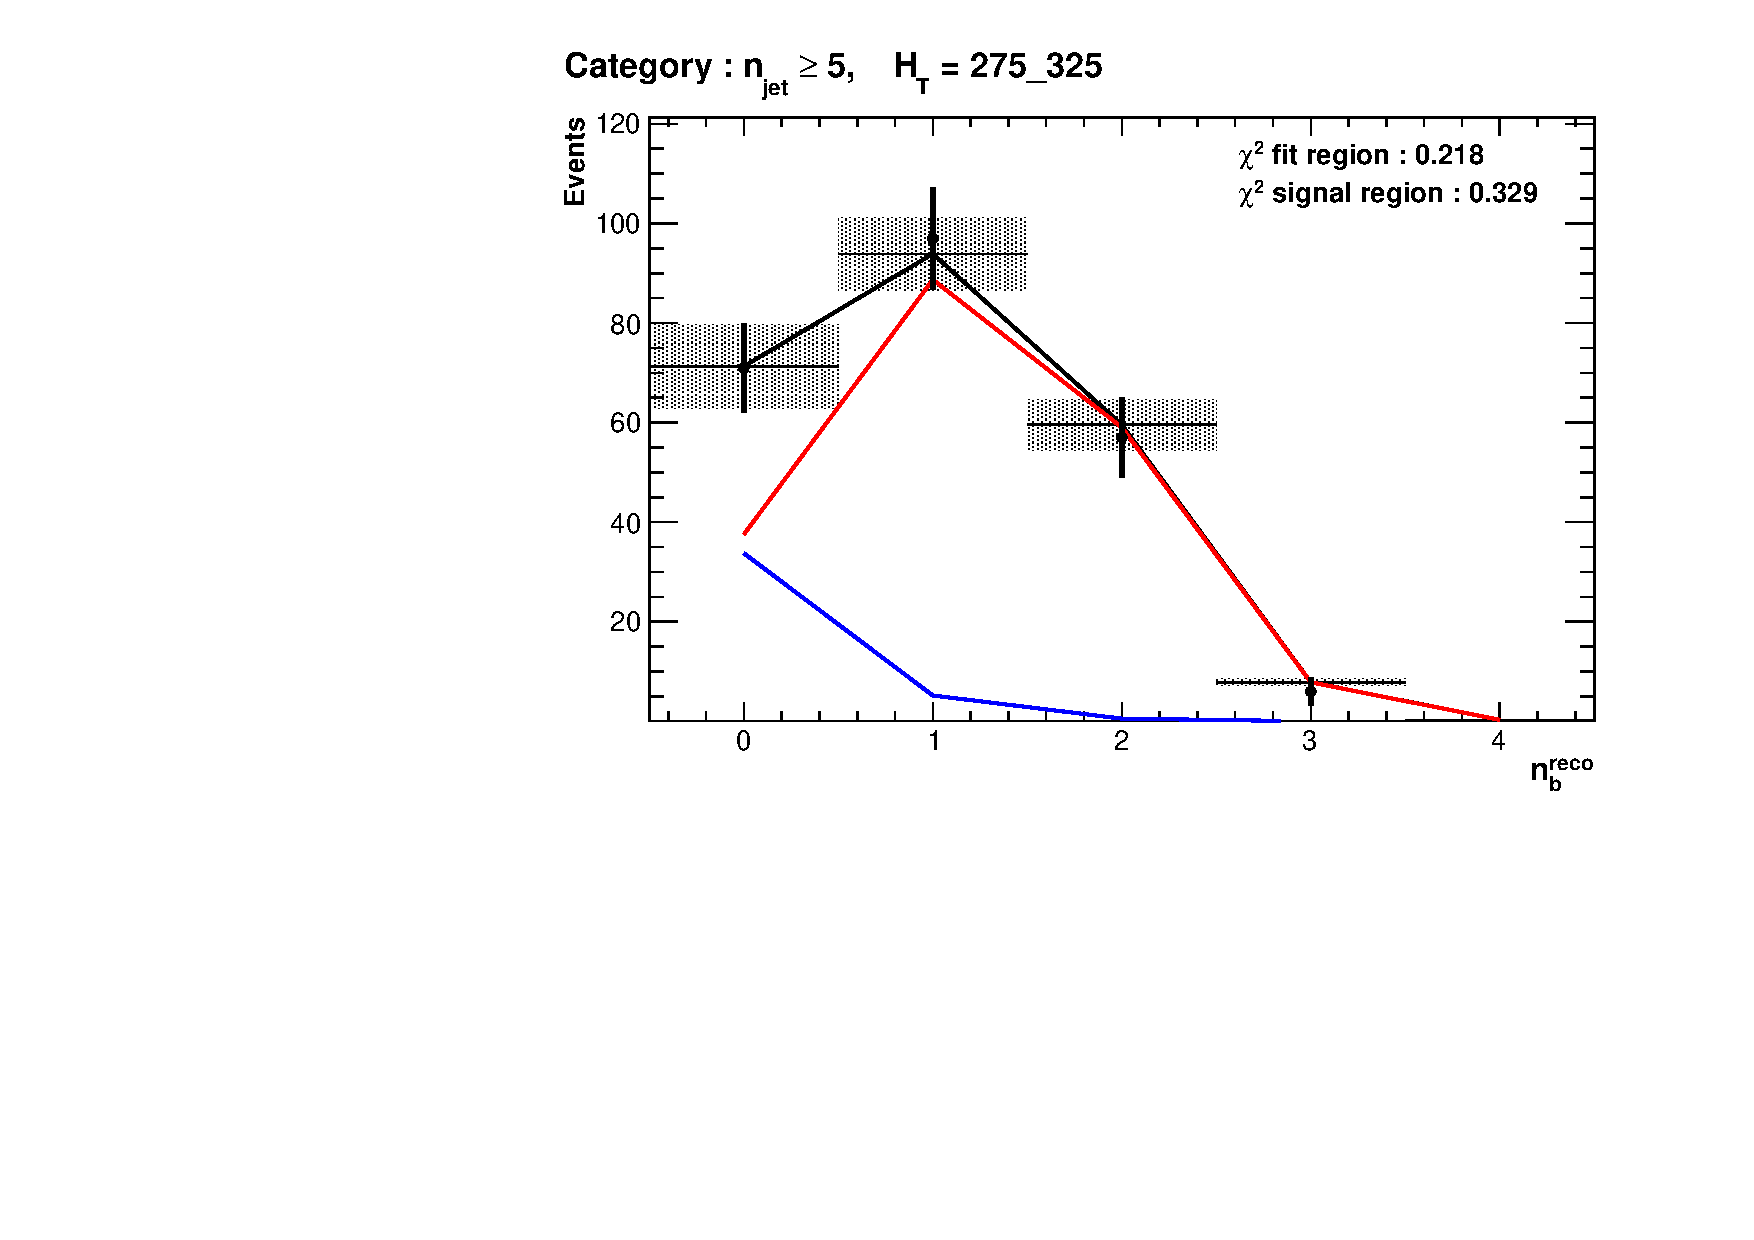
\includegraphics[width = 1.0\linewidth]{plots/ThesisPlots/Final_Fit_To_Data_Normal_Medium_HTBin_OneMuon_275_325_jet_mult_5.pdf}
\centering (a) $n_{jet} \geq$  5 , 275 $<$ \theht $<$ 325
\end{minipage}
\quad
\begin{minipage}[b]{0.51\linewidth}
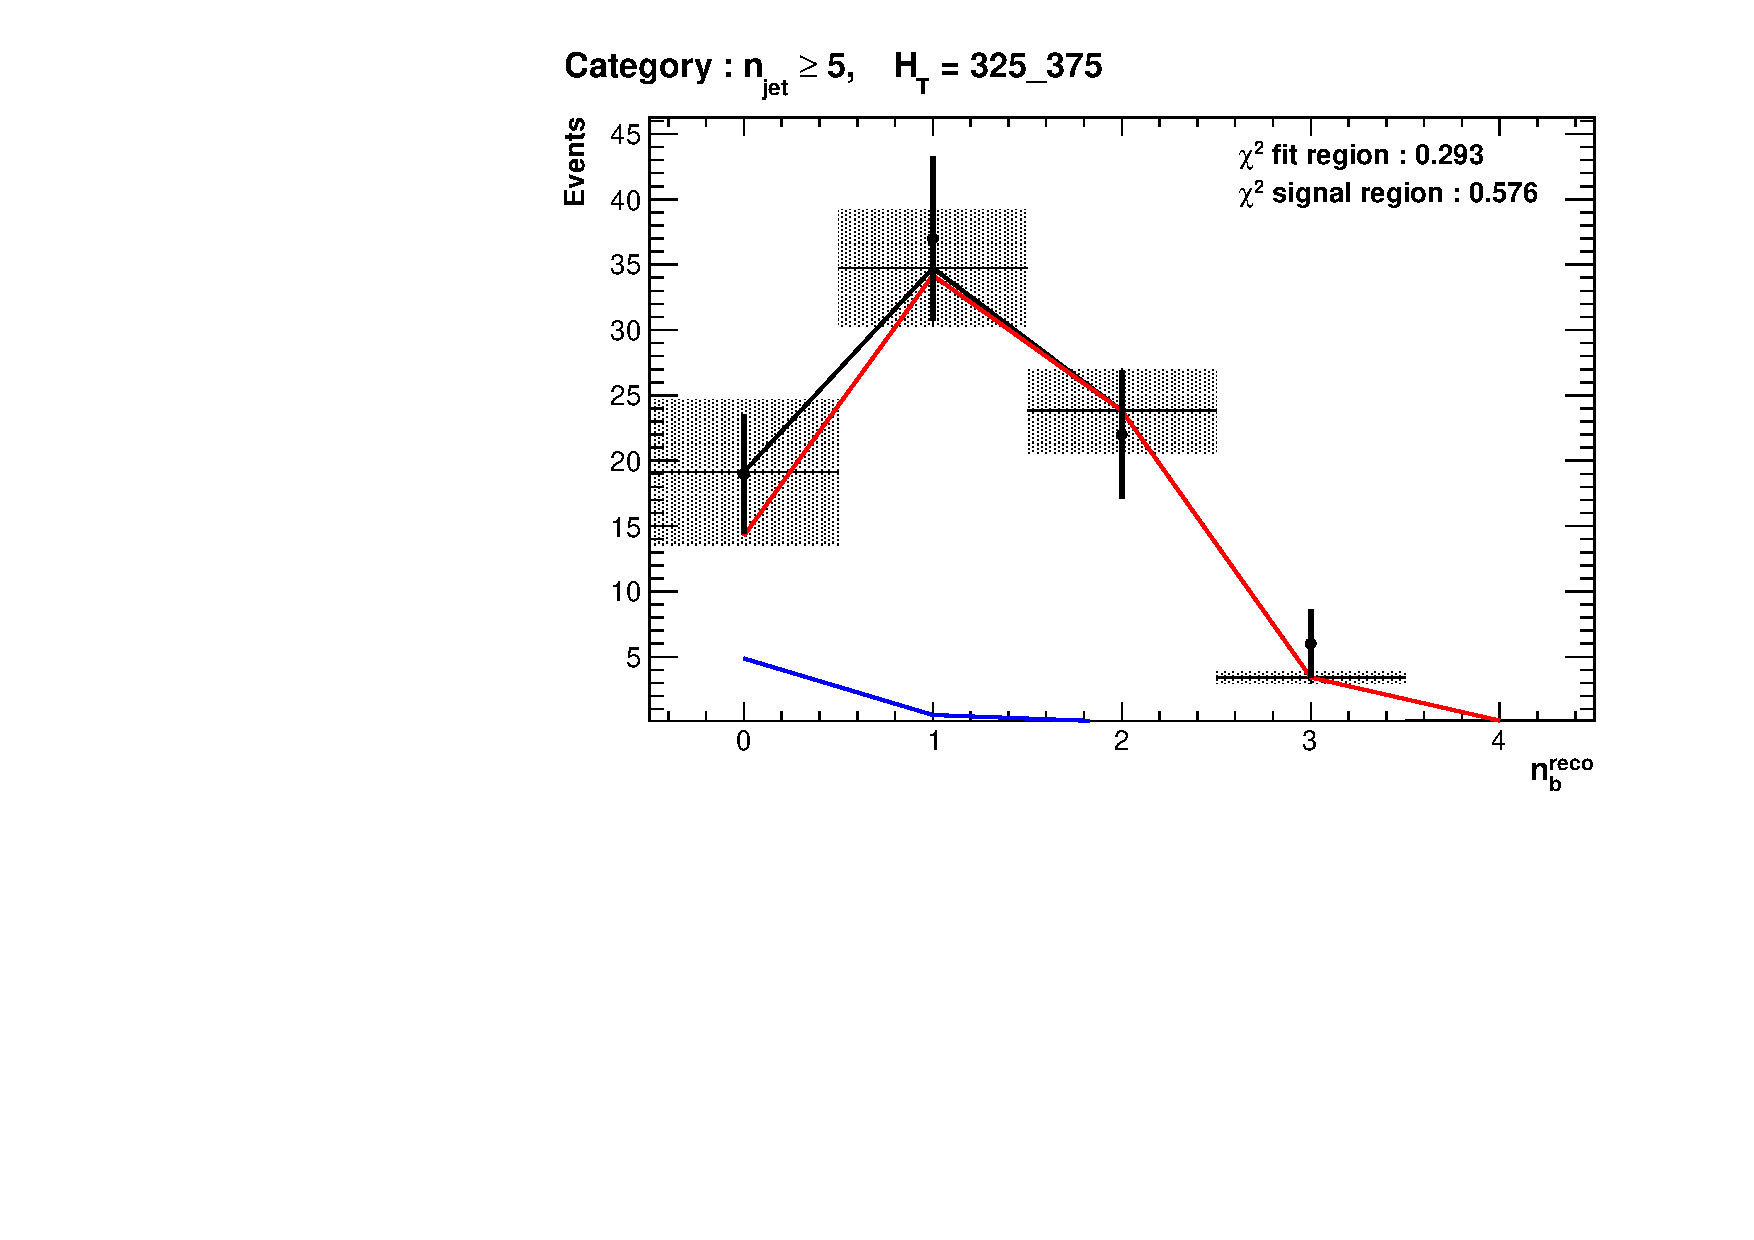
\includegraphics[width = 1.0\linewidth]{plots/ThesisPlots/Final_Fit_To_Data_Normal_Medium_HTBin_OneMuon_325_375_jet_mult_5.pdf}
\centering (b) $n_{jet} \geq$ = 5 , 325 $<$ \theht $<$ 375 
\end{minipage}
\quad
\begin{minipage}[b]{0.51\linewidth}
\centering
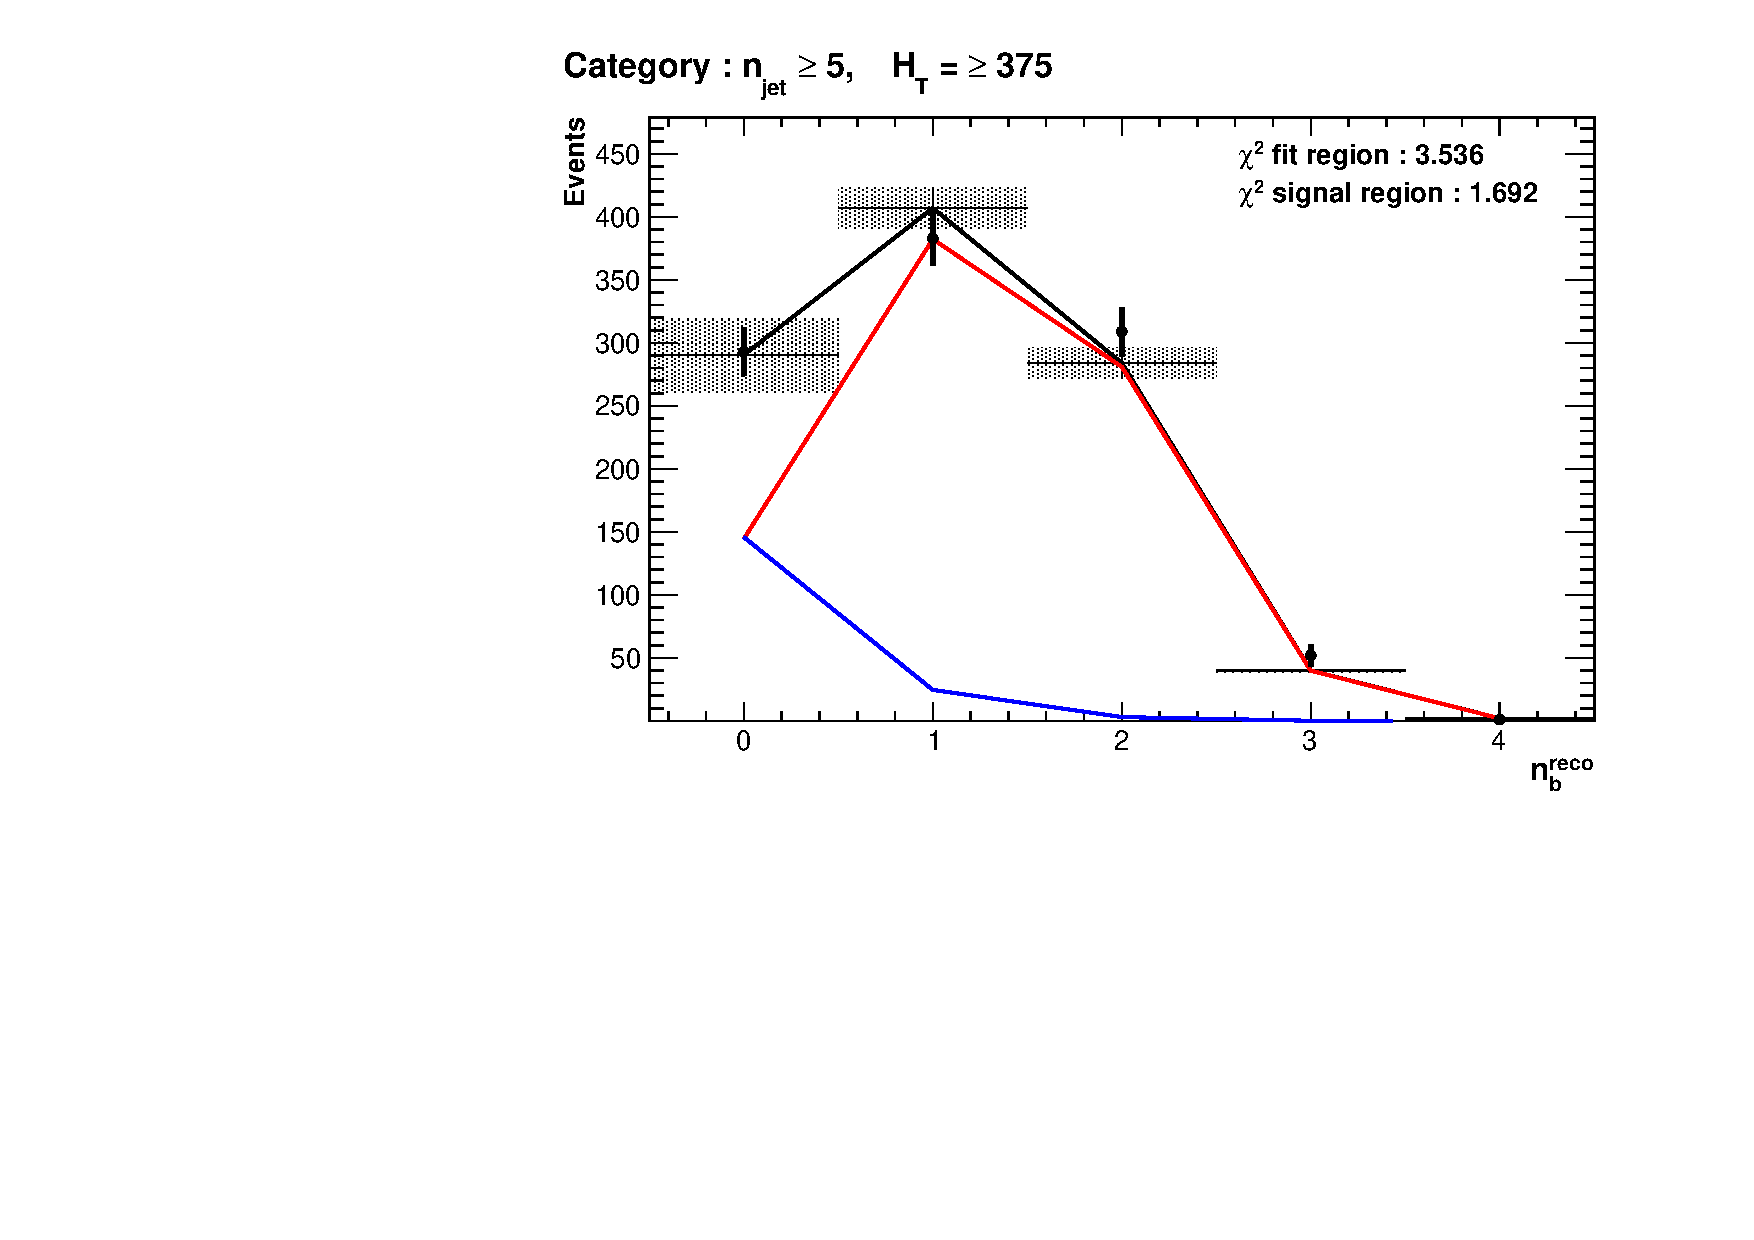
\includegraphics[width = 1.0\linewidth]{plots/ThesisPlots/Final_Fit_To_Data_Normal_Medium_HTBin_OneMuon_Template_375_jet_mult_5.pdf}
\centering (c) $n_{jet} \geq$ 5 , \theht $>$ 375 
\end{minipage}
\caption[The results of fitting the Z = 0 and Z = 2 templates to the $n_{b}^{reco}$ = 0, 1, 2 bins taken from data, for the $n_{jet} \geq 5$ category and medium \ac{CSV} working point.]{The results of fitting the Z = 0 and Z = 2 templates to the $n_{b}^{reco}$ = 0, 1, 2 bins taken directly from data, for the $n_{jet} \geq 5$ category and medium \ac{CSV} working point. The blue template represents Z = 0, while the red template represents Z = 2. The $\chi^{2}$ parameter displayed represents the goodness of fit to the low $n_{b}^{reco}$ (0-2) control region.}
\label{fig:template_data_med_njet5}
\end{figure}

The numerical results and extrapolation to the $n_{b}^{reco} =$3, 4 bins for all \theht and working points is shown in Table \ref{tab:template_datatable}.

\begin{table}[h!]
\begin{center}
\footnotesize
\begin{tabular*}{0.95\textwidth}{@{\extracolsep{\fill}}llll}
\cline{1-4}
\multicolumn{1}{c}{\theht} & 275-325 & 325-375 & $>$375 \\
\multicolumn{4}{c}{Loose working point} \\
\hline\hline
Data $n_{b} = 3$ & 838 & 394 & 717\\
Template $n_{b} = 3$ & $861.8 \pm 38.1$ & $372.1 \pm 18.4$ & $673.2 \pm 34.5$ \\
Data $n_{b} = 4$ & 81 & 43 & 81 \\
Template $n_{b} = 4$ & $78.5 \pm 5.8$ & $27.6 \pm 2.6$ & $78.6 \pm 3.3$ \\
\hline
\multicolumn{4}{c}{Medium working point} \\
\hline\hline
Data $n_{b} = 3$ & 137 & 79 & 152 \\
Template $n_{b} = 3$ & $131.2 \pm 4.3$ & $66.1 \pm 2.9$ & $137.8 \pm 5.7$ \\
Data $n_{b} = 4$ & 1 & 1 & 3 \\
Template $n_{b} = 4$ & $1.8 \pm 0.1$ & $0.9 \pm 0.1$ & $3.1 \pm 0.2$ \\
\hline
\multicolumn{4}{c}{Tight working point} \\
\hline\hline
Data $n_{b} = 3$ & 24 & 15 & 25 \\
Template $n_{b} = 3$ & $23.0 \pm 0.9$ & $12.9 \pm 0.6$ & $20.3 \pm 1.1$ \\
Data $n_{b} = 4$ & 0 & 0 & 1 \\
Template $n_{b} = 4$ & $0.1 \pm 0.1$ & $0.1 \pm 0.1$ & $0.2 \pm 0.1$ \\
\end{tabular*}
\end{center}
\caption[Summary of the fit predictions in the $n_{b}^{reco}$ signal region of the \mupjets control sample, for $n_{jet} = 3, = 4, \geq 5$. The fit region is $n_{b}^{reco}$ = 0, 1, 2 using 11.5 fb$^{-1}$ of data at $\sqrt{s} = 8$\TeV.]{Summary of the fit predictions in the $n_{b}^{reco}$ signal region of the \mupjets control sample, for $n_{jet} = 3, = 4, \geq 5$. The fit region is $n_{b}^{reco}$ = 0, 1, 2 using 11.4 fb$^{-1}$ of data at $\sqrt{s} = 8$\TeV. The uncertainties quoted on the template yields are purely statistical.}\label{tab:template_datatable}
\end{table}
\FloatBarrier

When this method is applied to the \mupjets control sample, it is expected that good agreement would be observed between prediction and observation (in the absence of signal contamination) if the procedure is valid. The good compatibility for all working points as shown in the table, demonstrate that this is the case. However no such assumptions can be made when applied to the signal region of the \alphat search.
 
 
\subsection{Application to the \alphat hadronic search region}
\label{subsec:templatedataresults}

As an accompaniment to the background estimation methods outlined in the \alphat search, the b-tag template method offers a complimentary way of testing the \ac{SM} only background hypothesis within the hadronic signal region of the search. In the presence of a natural \ac{SUSY} signature containing four underlying $\widetilde{b}$ or $\widetilde{t}$ squarks, which subsequently decay to t or b quarks, the number of reconstructed \nbreco = 3, $\geq 4$ events will be enhanced.

Figure \ref{fig:template_data_signal_njet5} show the  the results of the templates derived from simulation to each of the three \ac{CSV} working points, in the $n_{jet} \geq 5$, \theht $>$ 375 \GeV category.  Grey bands represent the statistical uncertainty of the fit combined in quadrature with the systematic uncertainties of varying the data to simulation scale factors up and down by their measured systematic uncertainties.  Additional fit results for other jet multiplicities are found in Appendix \ref{app:templatedata_signal}  

\begin{figure}[ht]
\footnotesize
\centering
\begin{minipage}[b]{0.51 \linewidth}
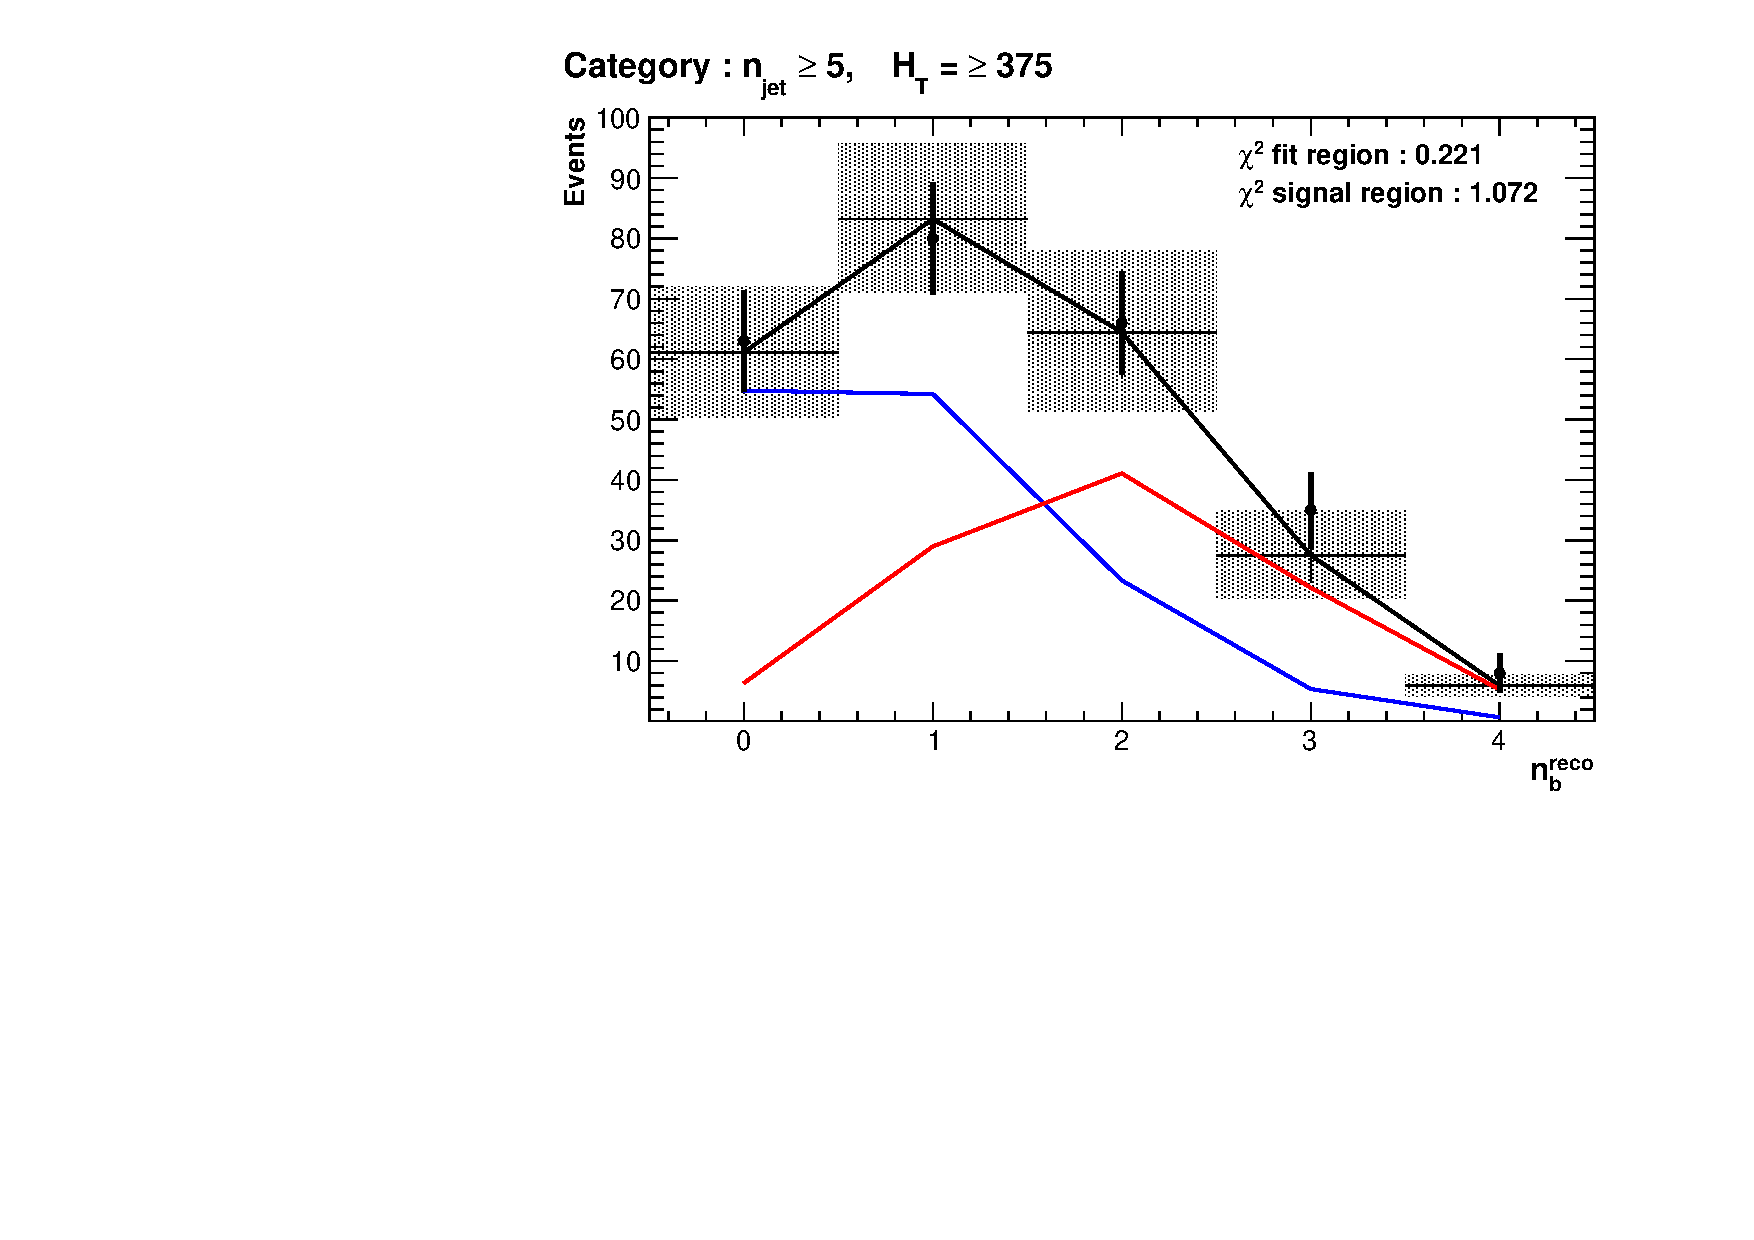
\includegraphics[width = 1.0\linewidth]{plots/TemplatesSignal/Final_Fit_To_Data_Normal_Loose_HTBin_Template_375_jet_mult_5.pdf}
\centering (a) Loose working point : $n_{jet} \geq$  5 , \theht $>$ 375
\end{minipage}
\quad
\begin{minipage}[b]{0.51\linewidth}
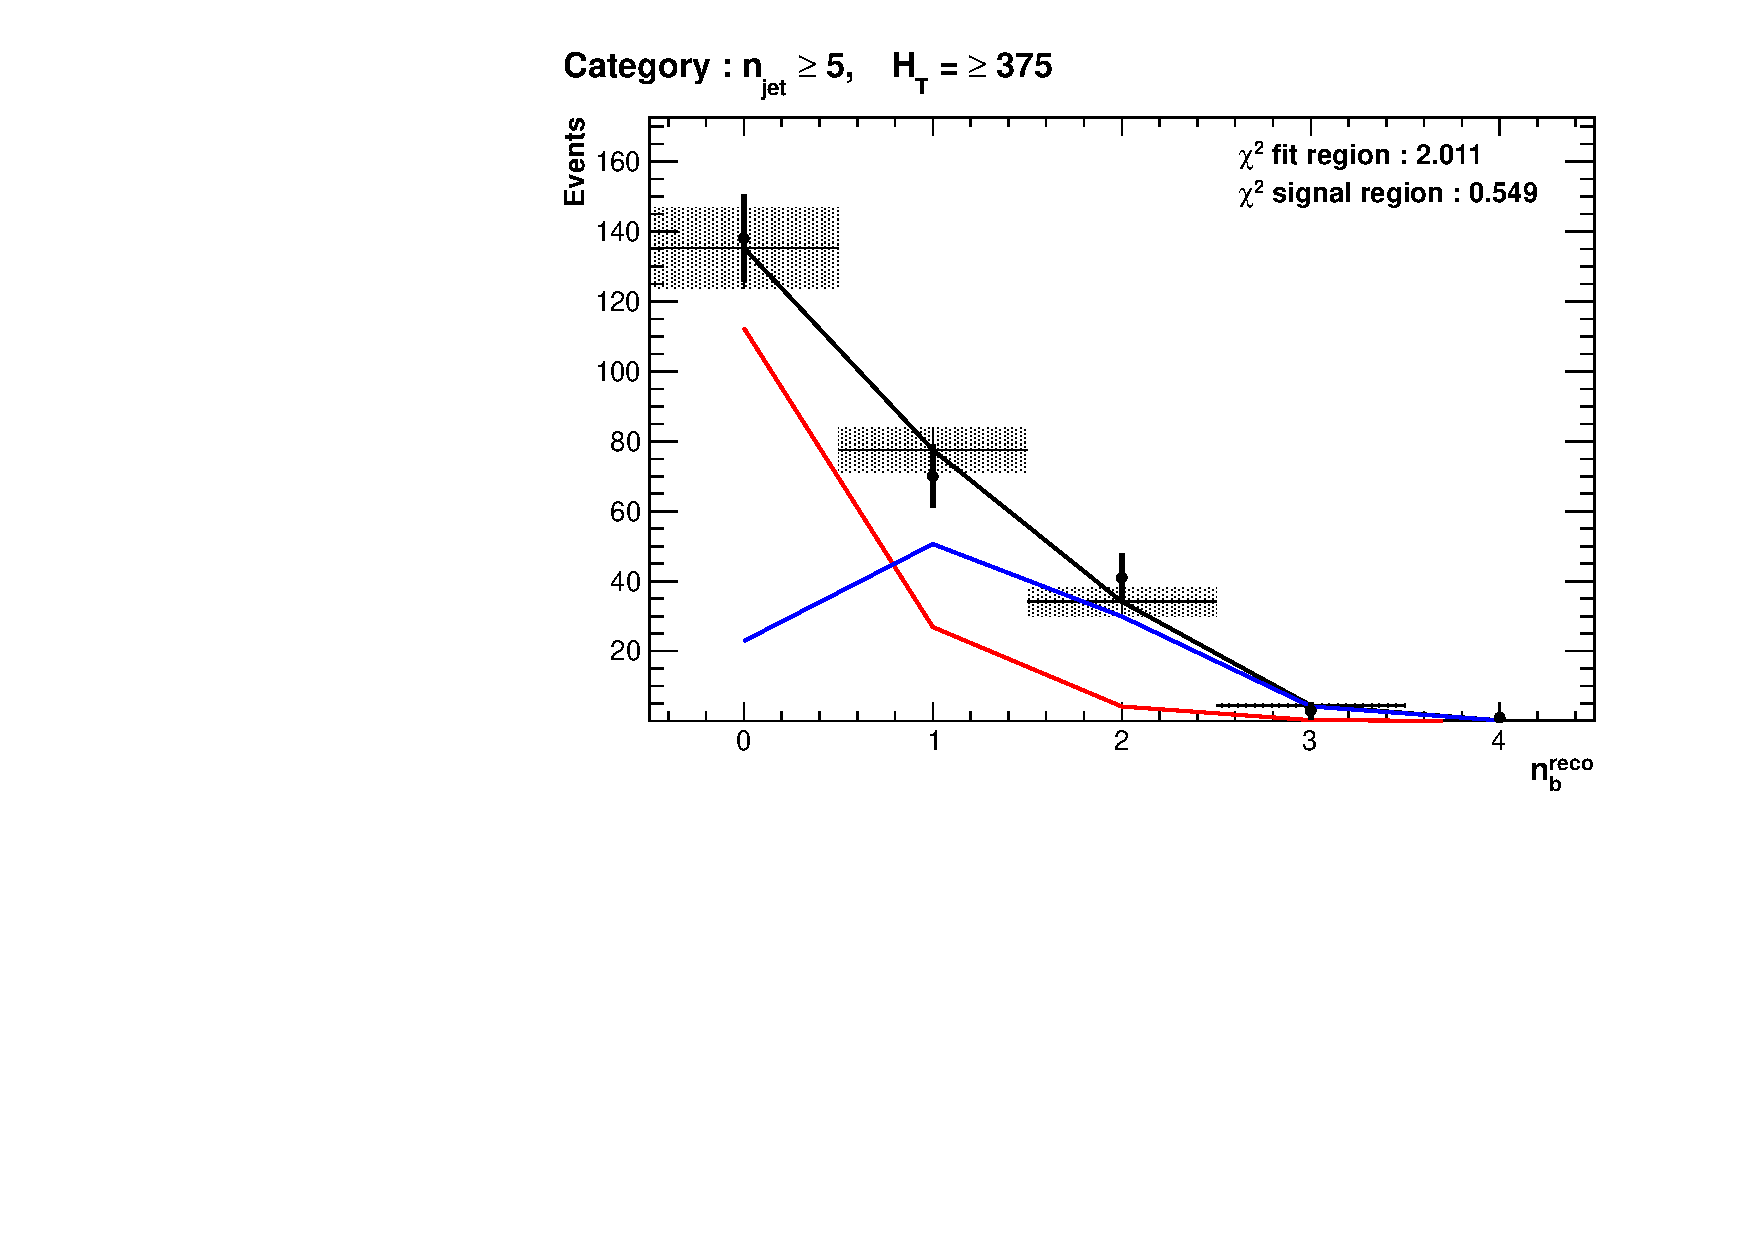
\includegraphics[width = 1.0\linewidth]{plots/TemplatesSignal/Final_Fit_To_Data_Normal_Medium_HTBin_Template_375_jet_mult_5.pdf}
\centering (b) Medium working point : $n_{jet} \geq$ 5 , \theht $>$ 375 
\end{minipage}
\quad
\begin{minipage}[b]{0.51\linewidth}
\centering
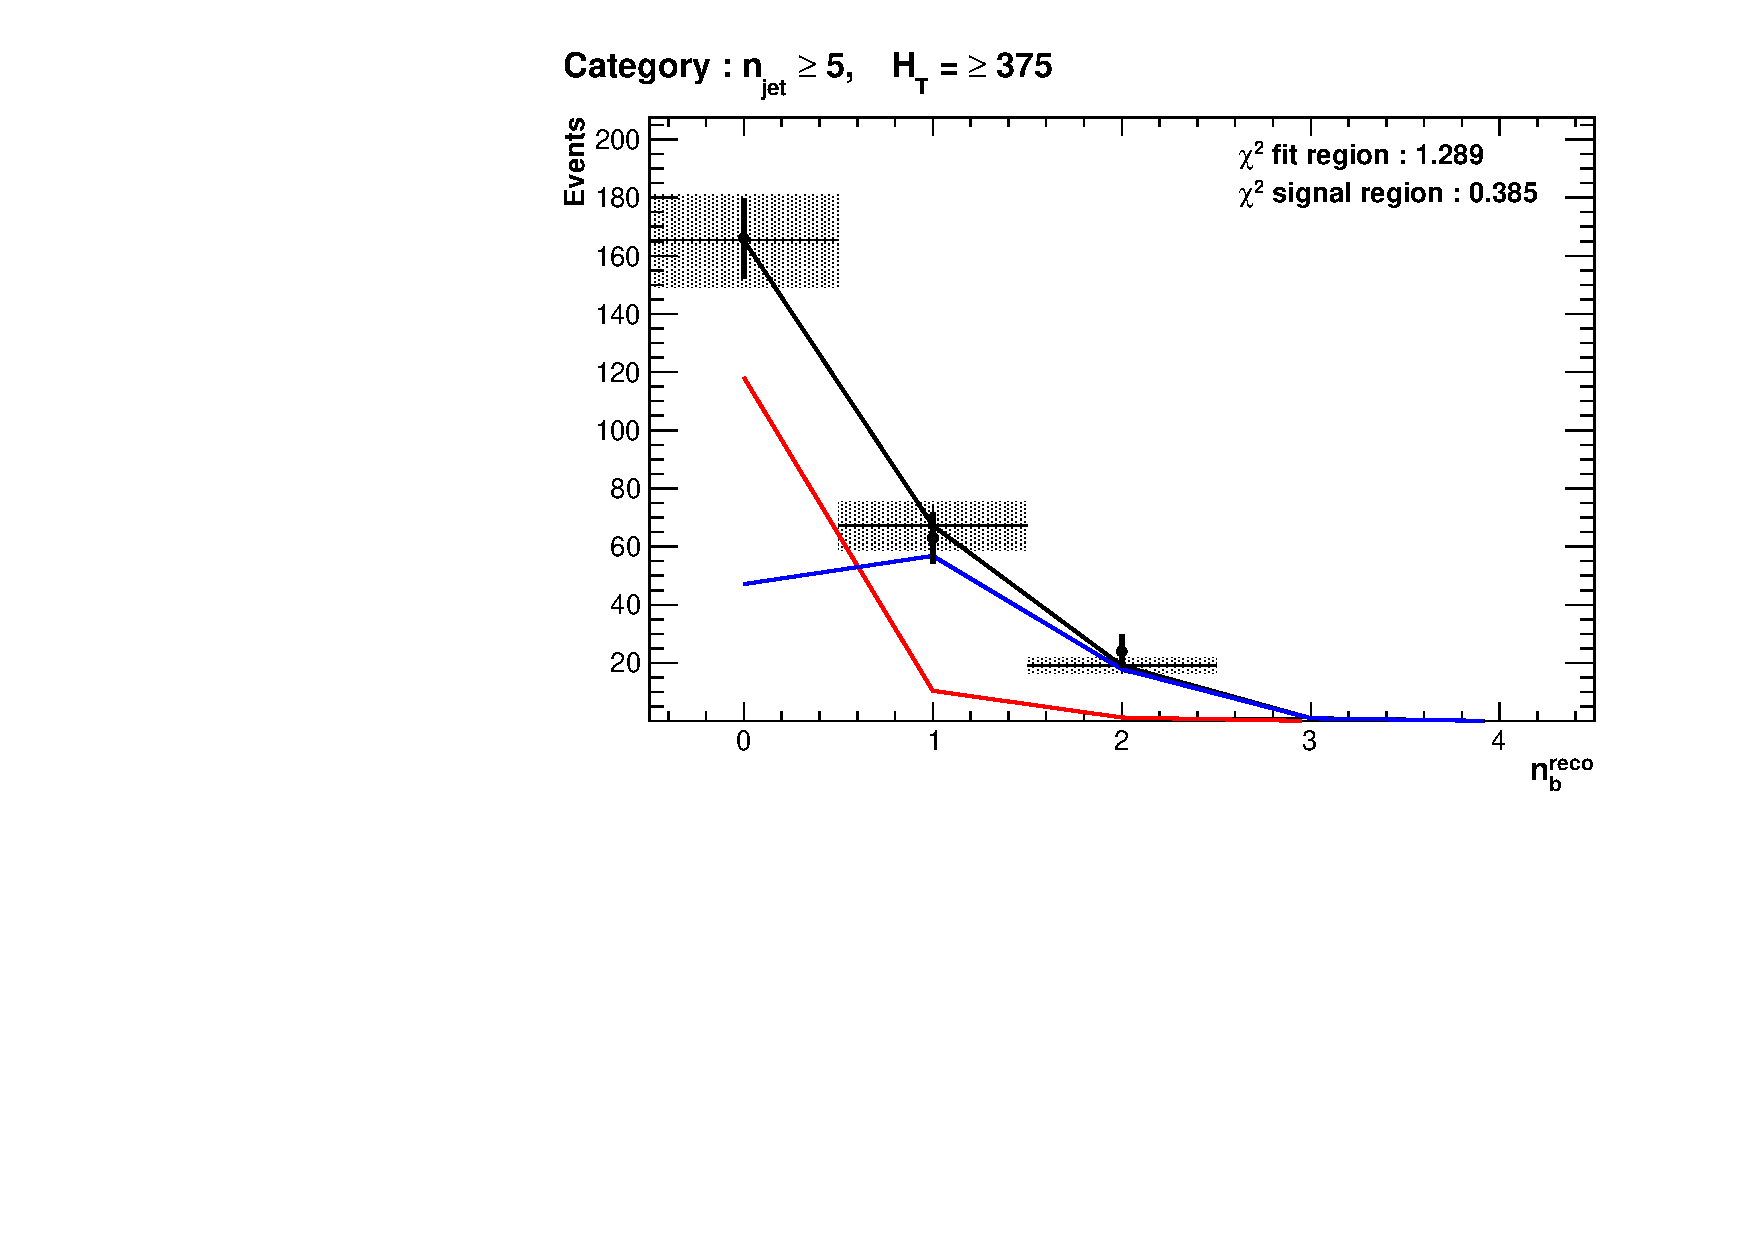
\includegraphics[width = 1.0\linewidth]{plots/TemplatesSignal/Final_Fit_To_Data_Normal_Tight_HTBin_Template_375_jet_mult_5.pdf}
\centering (c) Tight working point :  $n_{jet} \geq$ 5 , \theht $>$ 375 
\end{minipage}
\caption[The results of fitting the Z = 0 and Z = 2 templates to the $n_{b}^{reco}$ = 0, 1, 2 bins taken from data, in the $n_{jet} \geq 5$ and \theht $>$ 375 category for all \ac{CSV} working points.]{The results of fitting the Z = 0 and Z = 2 templates to the $n_{b}^{reco}$ = 0, 1, 2 bins taken from data, in the $n_{jet} \geq 5$ and \theht $>$ 375 category for all \ac{CSV} working points. The blue template represents Z = 0, while the red template represents Z = 2. The $\chi^{2}$ parameter displayed represents the goodness of fit to the low$ n_{b}^{reco}$ (0-2) control region.}
\label{fig:template_data_signal_njet5}
\end{figure}

The numerical results and extrapolation to the $n_{b}^{reco} =$3, 4 bins for all \theht and working points are shown in Table \ref{tab:template_signal_table}. No excess of data is found and predictions from this method are found to be compatible with the \alphat maximum likelihood fit results from Table \ref{tab:fitsdata}.

\begin{table}[h!]
\begin{center}
\footnotesize
\begin{tabular*}{0.95\textwidth}{@{\extracolsep{\fill}}llll}
\cline{1-4}
\multicolumn{1}{c}{\theht} & 275-325 & 325-375 & $>$375 \\
\multicolumn{4}{c}{Loose working point} \\
\hline\hline
Data $n_{b} = 3$ & 198 & 85 & 126\\
Template $n_{b} = 3$ & $207.1 \pm 33.3$ & $103.4 \pm 10.9$ & $124.98 \pm 16.2$ \\
Data $n_{b} = 4$ & 15 & 9 & 16 \\
Template $n_{b} = 4$ & $15.9 \pm 3.7$ & $8.05 \pm 1.2$ & $13.1 \pm 2.2$ \\
\hline
\multicolumn{4}{c}{Medium working point} \\
\hline\hline
Data $n_{b} = 3$ & 28 & 15 & 12 \\
Template $n_{b} = 3$ & $24.4 \pm 1.7$ & $12.7 \pm 1.2$ & $19.9 \pm 2.8$ \\
Data $n_{b} = 4$ & 1 & 0 & 2 \\
Template $n_{b} = 4$ & $0.3 \pm 0.2$ & $0.3 \pm 0.1$ & $0.5 \pm 0.2$ \\
\hline
\multicolumn{4}{c}{Tight working point} \\
\hline\hline
Data $n_{b} = 3$ & 5 & 2 & 0 \\
Template $n_{b} = 3$ & $4.03 \pm 0.3$ & $2.4 \pm 0.3$ & $3.1 \pm 0.3$ \\
Data $n_{b} = 4$ & 1 & 0 & 0 \\
Template $n_{b} = 4$ & $0.1 \pm 0.1$ & $0.1 \pm 0.1$ & $0.0 \pm 0.1$ \\
\end{tabular*}
\end{center}
\caption[Summary of the fit predictions in the $n_{b}^{reco}$ signal region of the \mupjets control sample, for $n_{jet} = 3, = 4, \geq 5$. The fit region is $n_{b}^{reco}$ = 0, 1, 2 using 11.5 fb$^{-1}$ of data at $\sqrt{s} = 8$\TeV.]{Summary of the fit predictions in the $n_{b}^{reco}$ signal region of the \mupjets control sample, for $n_{jet} = 3, = 4, \geq 5$. The fit region is $n_{b}^{reco}$ = 0, 1, 2 using 11.7 fb$^{-1}$ of data at $\sqrt{s} = 8$\TeV. The uncertainties quoted on the template yields are purely statistical.}\label{tab:template_signal_table}
\end{table}
\FloatBarrier


\section{Summary}
\label{subsec:templateconclusions}

A \ac{SUSY} signature such as one from gluino-induced third-generation squark production, would result in a final state with an underlying b-quark content greater than two. In order to be able to discriminate such signatures from the \ac{SM} background, templates are generated based on a parameterisation of the number of the \ac{SM} processes, where the underlying b-quarks per event is typically zero or two. These templates are then fit to data in a low $n_{b}^{reco}$ (0-2) control region in order to extrapolate a prediction in a high $n_{b}^{reco}$ (3-4) signal region. This approach is built upon the assumptions that the defined control region is almost entirely free of any possible signal contamination from either a third generation \ac{SUSY} signal, or other possible event topologies with a small number of b quarks in the final state.

The method was demonstrated both in simulation and also in data, using the \ac{SM} enriched \mupjets selection from the \alphat search, to prove conceptually and experimentally that the method is valid and there is adequate control over the efficiency and mis-tagging rates in data for all working points of the \ac{CSV} tagger. Additionally this method was also applied to the \alphat analysis signal region, where good agreement is observed between the predictions from the template extrapolations, observations in data and the background estimation method of the \alphat analysis.

